\setcounter{section}{5}
\section{ITB: Gauß-Pyramide}
\begin{figure}
	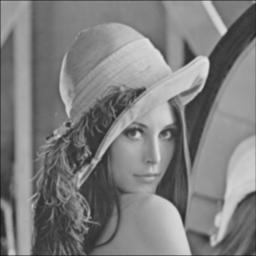
\includegraphics[]{A6/1.jpg}
	
\includegraphics[]{A6/2.jpg}
	
\includegraphics[]{A6/3.jpg}
	
\includegraphics[]{A6/4.jpg}
	
\includegraphics[]{A6/5.jpg}
	
\includegraphics[]{A6/6.jpg}
	
\includegraphics[]{A6/7.jpg}
	\caption{Reduce}
\end{figure}

\begin{figure}
	\centering
	\begin{subfigure}{.49\textwidth}
		\centering
		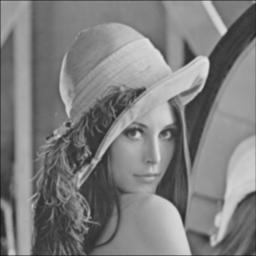
\includegraphics[width=.99\linewidth]{A6/1.jpg}
		
\includegraphics[width=.99\linewidth]{A6/2.jpg}
		\caption{Reduce}
	\end{subfigure}
	\begin{subfigure}{.49\textwidth}
		\centering
		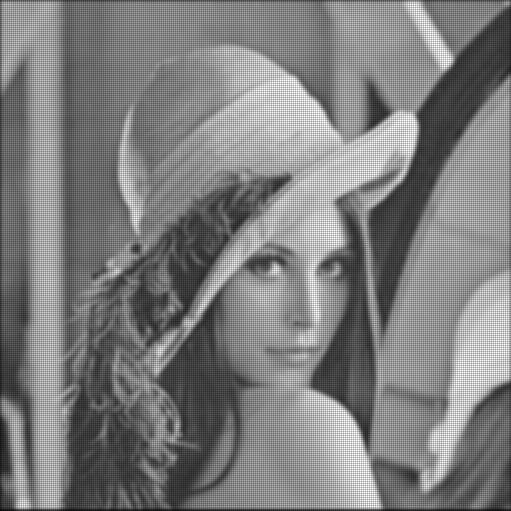
\includegraphics[width=.99\linewidth]{A6/expand1.jpg}
		
\includegraphics[width=.99\linewidth]{A6/expand2.jpg}
		\caption{Expand}
	\end{subfigure}
\end{figure}